% sections/methodology_and_design.tex

\section{Methodology and Design}

This chapter describes the methodology used to evaluate and address the
``noisy neighbor'' isolation problem in sidecarless (eBPF-based) service
mesh architectures. Rather than relying on simulation, the project takes an
empirical, systems-level approach, building a controlled containerized
testbed and measuring the real behaviour of the Linux kernel under
contention.

\subsection{Approach and Methodology}
To isolate kernel-level effects from the noise that a full orchestrator
like Kubernetes would introduce, the project uses a minimal container
networking setup built directly on \texttt{runc} and Linux network
namespaces, rather than Docker or a managed cluster. This gave more direct
control over CPU placement, IRQ affinity, and cgroup configuration than a
higher-level platform would have allowed. The work progressed through three
broad phases:

\begin{enumerate}
    \item \textbf{Baseline Architectural Profiling.} Baseline latency and
    throughput figures were established by comparing a traditional
    sidecar-proxy data plane against a sidecarless eBPF data plane. This
    phase varied the number of co-located noisy neighbours, CPU core
    allocation, and the transport protocol (HTTP, TCP, UDP, gRPC) to see
    how badly, and under what conditions, the isolation deficit actually
    shows up.
    \item \textbf{Dual-Direction Ablation Study.} Two candidate mitigation
    strategies were investigated in parallel before committing to one:
    \begin{itemize}
        \item \textit{Direction 1 (Architectural):} a static priority-tier
        QoS scheme, modelled loosely on production container-networking
        designs such as Alibaba's Terway-QoS \cite{aliyun2024terway}, was
        compared against a dynamic rate limiter driven by an adaptive
        feedback controller.
        \item \textit{Direction 2 (Micro-architectural):} Beeswax-style
        stall-hiding \cite{shahinfar2026dont} was applied to the eBPF
        limiter's own hot path, to test whether reducing the limiter's
        internal memory-access latency would meaningfully affect
        end-to-end tail latency.
    \end{itemize}
    \item \textbf{Comprehensive Workload Matrix.} The architecture that
    performed best in the ablation study was then evaluated against seven
    adversarial and real-world traffic patterns, to check that the result
    wasn't an artefact of the synthetic flood used in the earlier phases.
\end{enumerate}

\subsection{System Architecture}
The mitigation system separates the cheap, latency-critical decision from
the expensive control logic, splitting the work across the kernel and
user space. Figure \ref{fig:architecture} shows the traffic lifecycle
across four layers.

\begin{figure}[htbp]
    \centering
    \includegraphics[width=\textwidth]{images/System-Arch.jpeg}
    \caption{End-to-End System Architecture for Sidecarless eBPF Enforcement}
    \label{fig:architecture}
\end{figure}

\begin{itemize}
    \item \textbf{Traffic Generation (Layer 1):} Traffic entering the host
    is a mix of legitimate requests and high-rate floods from attacker
    nodes (UDP/TCP), generated by separate network namespaces to keep the
    two traffic sources clearly distinguishable in the measurements.
    \item \textbf{Host Linux Kernel Data Plane (Layer 2):} Traffic crosses
    a Linux bridge (\texttt{br-mesh}) before reaching the eBPF enforcement
    point attached at the \texttt{tc} ingress hook. The hook itself only
    does a fast state lookup and a budget check, following the general
    pattern of early, in-kernel packet filtering used in prior eBPF/XDP
    rate-limiting work \cite{tolay2025ebpf}. Per-tenant token-bucket state
    is kept in a \texttt{BPF\_MAP\_TYPE\_PERCPU\_HASH} map. By sharding state
    per CPU core, this design eliminates cross-core spinlock contention on
    \texttt{htab\_lock\_bucket} identified during baseline root-cause analysis,
    reducing map access overhead to a negligible per-core L1/L2 cache lookup
    cost \cite{netflix2024noisy}. Packets within budget are forwarded; packets
    over budget are dropped at the hook with \texttt{TC\_ACT\_SHOT}.
    \item \textbf{User Space Control Plane (Layer 3):} A Python controller
    process polls the kernel telemetry maps (packet-hit counters and
    lock-wait histograms), computes an updated rate limit $r_i$, and writes
    it back into the kernel-side map. Driving this off in-kernel telemetry
    rather than, say, polling application-level metrics was a deliberate
    choice, intended to keep the feedback loop closer to where the actual
    contention is happening \cite{netflix2024noisy}.
    \item \textbf{Isolated Container Namespaces (Layer 4):} Traffic that
    clears the kernel-side budget check is delivered to the victim
    container as normal.
\end{itemize}

\subsection{The Dynamic Rate Limiter}
The control-plane logic is built around an adaptive feedback controller
informed by leader-follower contention dynamics. The controller dynamically
adjusts the bandwidth ceiling of non-legitimate (follower) tenants based on
real-time kernel contention telemetry.

Bandwidth rate limits $r^*(H)$ are computed using a smooth Hill-type sigmoid decay function:
\begin{equation}
    r^*(H) = \max \left( r_{\min}, \min \left( r_{\max}, \frac{r_{\max}}{1 + \left(\frac{H}{H_0}\right)^\gamma} \right) \right)
\end{equation}
where $r_{\max} = 50\,\text{MB/s}$ is the maximum baseline bandwidth, $r_{\min} = 500\,\text{KB/s}$
is the rate floor, $H$ is the observed eBPF map update frequency (hits/sec), and
$H_0 = 15{,}000\,\text{hits/sec}$ and $\gamma = 2.0$ are empirically tuned hyperparameters
corresponding to the contention inflection point identified during baseline profiling.

To minimize control-plane overhead, the controller uses an adaptive polling interval
$dC/dt$ based on the rate of change of kernel contention (Figure \ref{fig:solver}).

\begin{figure}[htbp]
    \centering
    \includegraphics[width=0.8\textwidth]{images/Dynamic-Stackelberg-Solver.jpeg}
    \caption{Execution Loop of the Dynamic Rate-Limiting Solver with Adaptive Polling}
    \label{fig:solver}
\end{figure}

\begin{enumerate}
    \item \textbf{Telemetry Ingestion.} The controller reads the current
    packet-hit count and lock-wait latency from the kernel maps.
    \item \textbf{Adaptive Polling.} Instead of polling on a fixed timer,
    the controller estimates the rate of change of contention,
    $dC/dt$, from consecutive readings, and adjusts its own polling
    interval accordingly:
    \begin{itemize}
        \item If contention is rising sharply, the interval drops to
        20\,ms so the controller can react almost immediately.
        \item Under moderate, fluctuating contention, it settles at a
        200\,ms baseline.
        \item When contention is flat and low, it relaxes to 1000\,ms,
        since there's little benefit to polling aggressively when nothing
        is changing.
    \end{itemize}
    \item \textbf{Rate Computation.} Traffic is classified by source IP
    into one of two roles. Known legitimate IPs are treated as the
    leader and are left uncapped ($r = 0$); everything else is treated as
    the follower, and a new bandwidth limit $r^*(H)$ is computed as a
    function of the observed hit rate $H$.
    \item \textbf{Enforcement and Sleep.} The computed limits are written
    into the kernel maps, and the controller sleeps for whatever interval
    was chosen in step 2 before repeating the loop.
\end{enumerate}

\subsection{Tools Used}
The following tools were used for load generation and kernel-level
profiling:
\begin{itemize}
    \item \textbf{\texttt{wrk2} / \texttt{fortio}:} used for constant-
    throughput load generation and tail-latency measurement across all
    four protocols tested. \texttt{wrk2} in particular was chosen because
    it is designed to avoid coordinated omission, a known source of
    distortion in naive load-testing tools.
    \item \textbf{\texttt{bpftrace}:} used to trace \texttt{sched\_wakeup}
    and \texttt{sched\_switch} to measure CFS run-queue latency, following
    the general methodology described in Netflix's eBPF-based
    noisy-neighbour work \cite{netflix2024noisy}.
    \item \textbf{eBPF \textit{ktime} histograms:} a custom in-kernel
    histogram map used to measure spinlock wait time directly, cross-
    checked against a \texttt{bpftrace} kprobe on \texttt{htab\_lock\_bucket}
    to make sure the two measurements agreed.
    \item \textbf{\texttt{mpstat}:} used to monitor per-core CPU
    utilisation and softirq load during flood conditions.
\end{itemize}

\subsection{Preliminary Results and Discussion}

Baseline testing across $N=5$ averaged runs showed a clear isolation problem in the
unmodified sidecarless mesh: P99 tail latency increased by more than 100\% under
high-intensity flooding, a degradation that the sidecar-proxy baseline did
not show under the same conditions (Figure \ref{fig:baseline_avg}). Scaling
the topology up to ten nodes ($N=5$ runs) showed that this isolation deficit gets worse
as the number of noisy neighbours increases (Figure
\ref{fig:baseline_nodes}). An earlier single-run version of this plot was
replaced here with an averaged $N=5$ version once it became clear that a
single run wasn't a reliable basis for the comparison.

\begin{figure}[htbp]
    \centering
    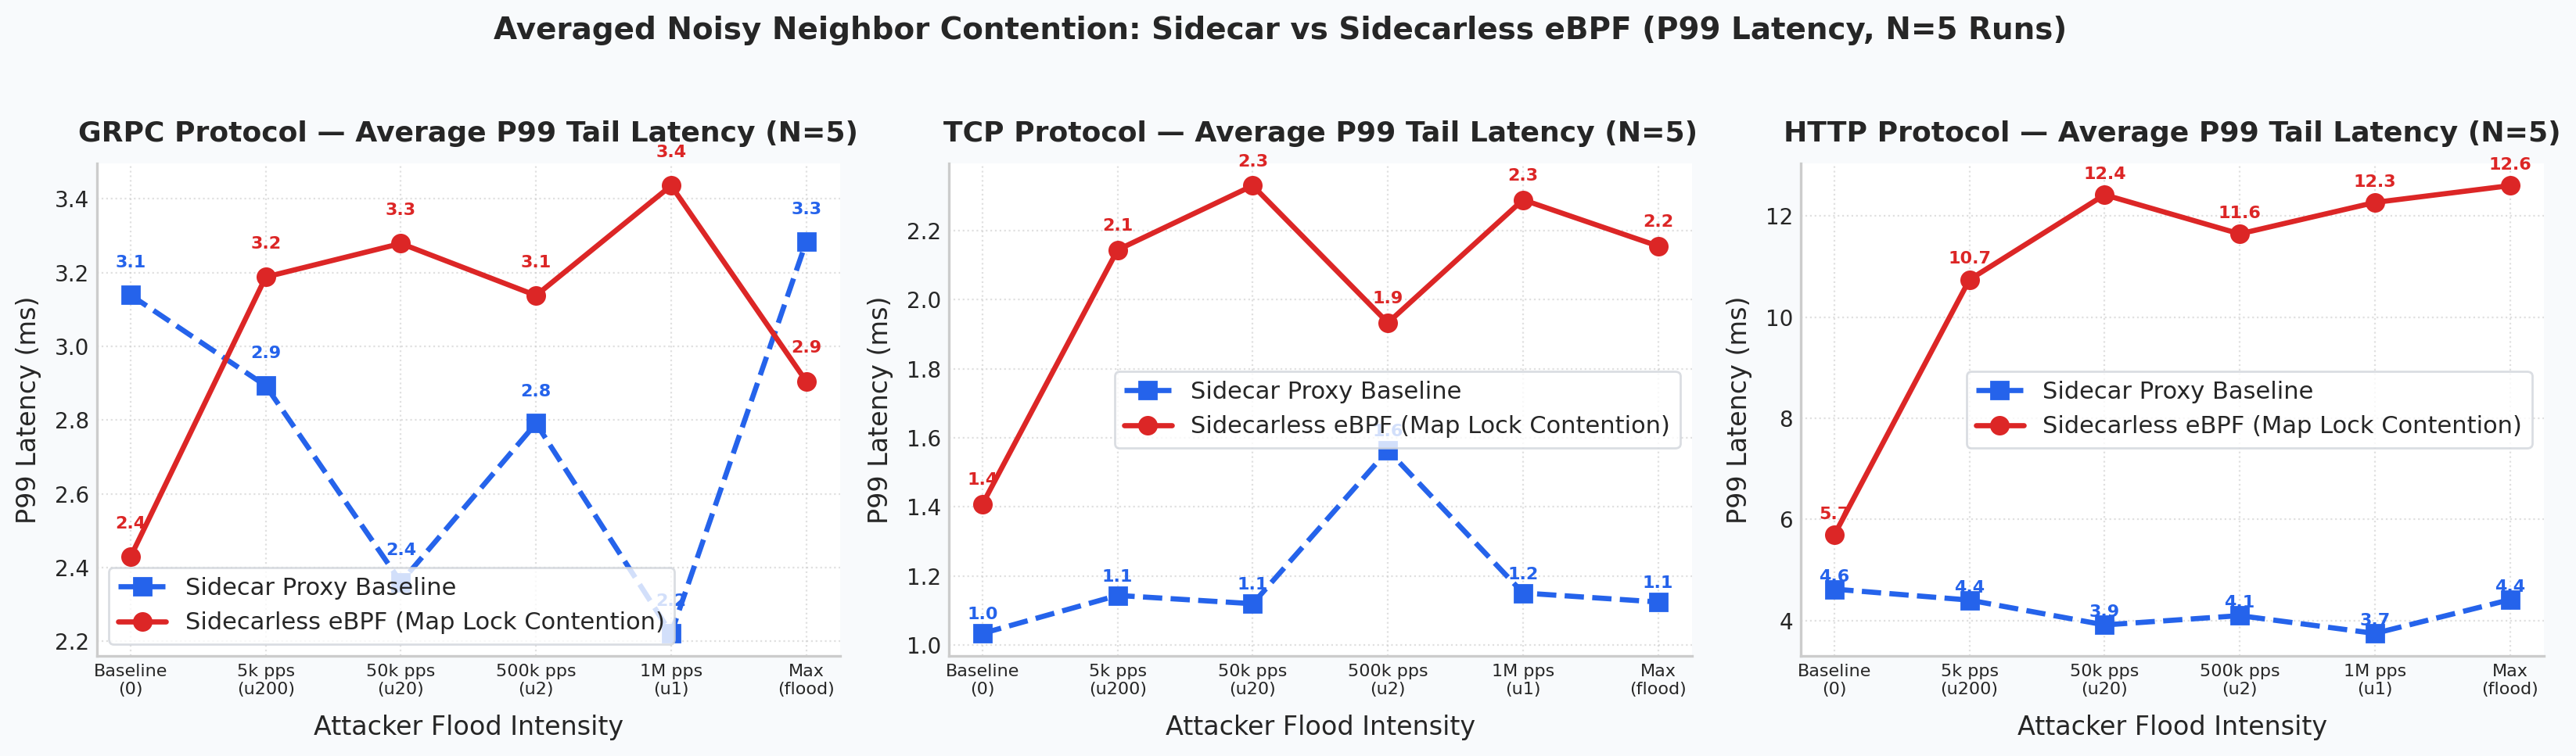
\includegraphics[width=\textwidth]{images/Sidecar vs Sidecarless eBPF (N=5 Runs).png}
    \caption{Averaged Noisy Neighbor Contention: Sidecar vs Sidecarless eBPF (N=5 Runs)}
    \label{fig:baseline_avg}
\end{figure}

\begin{figure}[htbp]
    \centering
    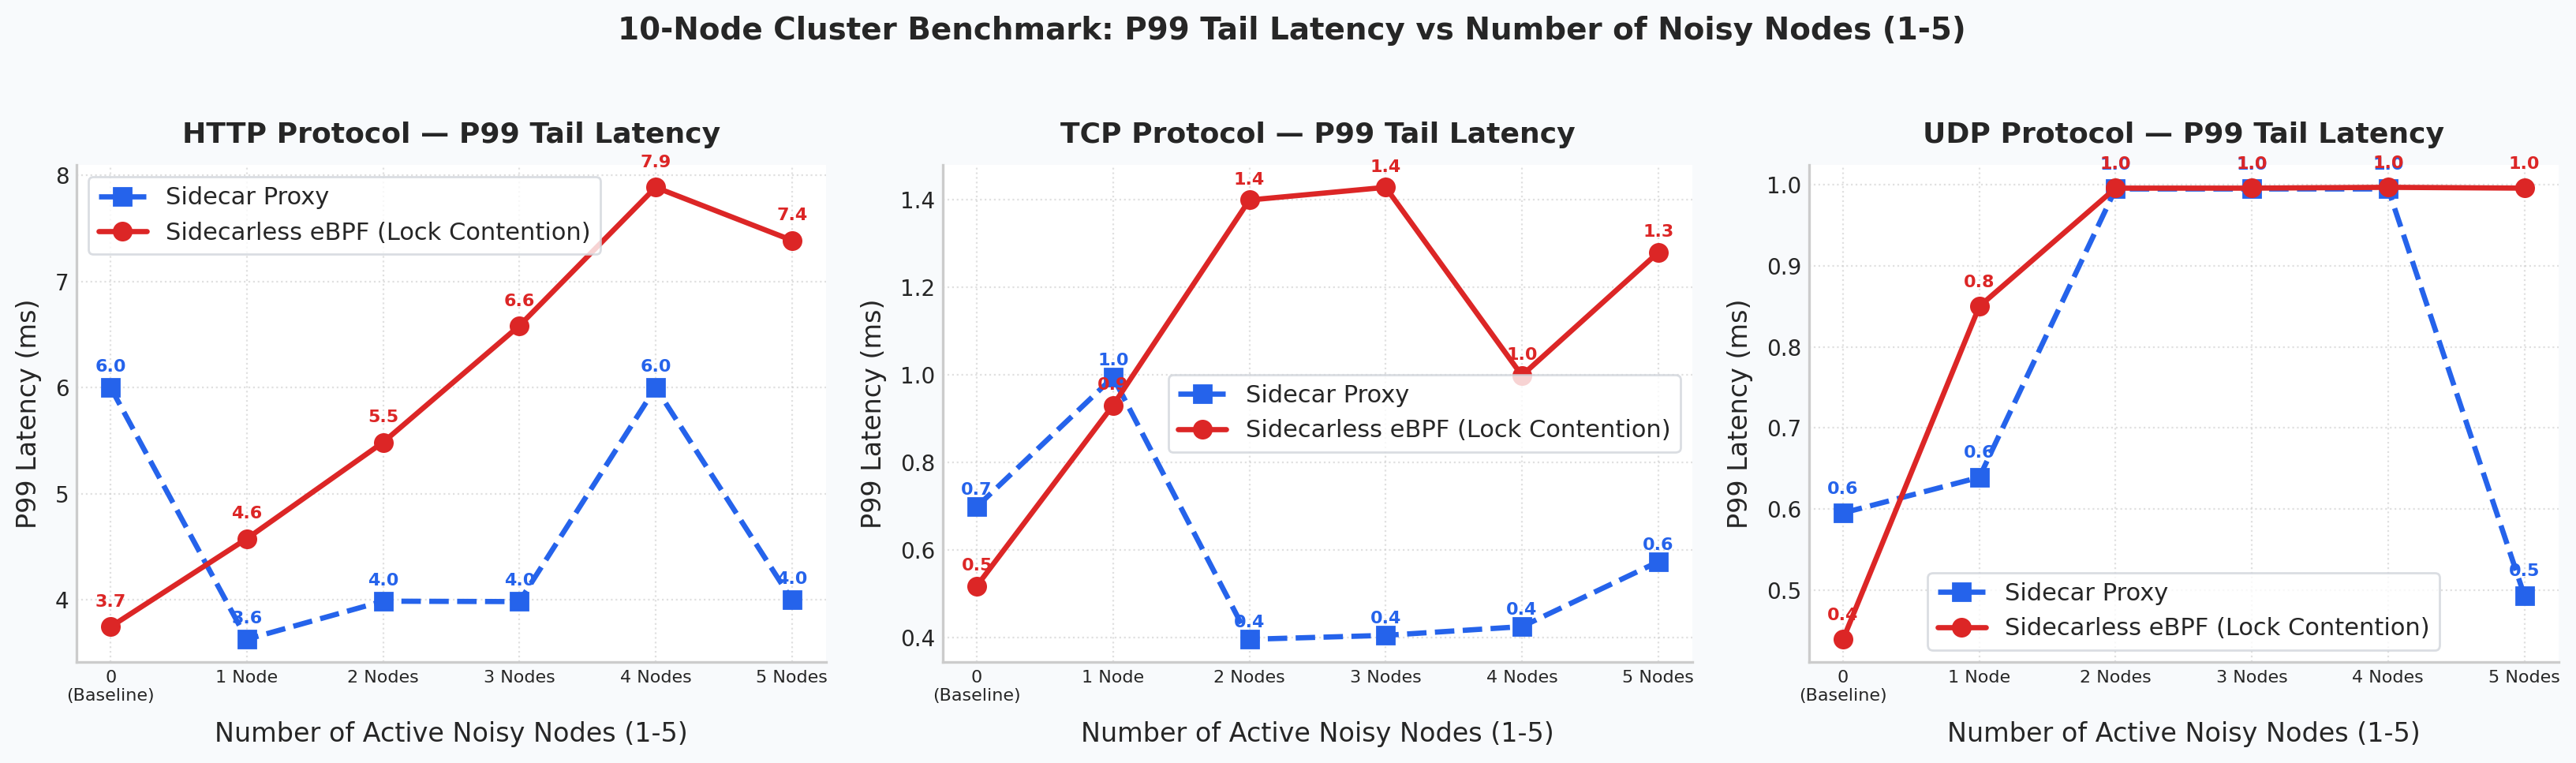
\includegraphics[width=\textwidth]{images/P99 Tail Latency vs Number of Noisy Nodes.png}
    \caption{10-Node Cluster Benchmark: P99 Tail Latency vs Number of Noisy Nodes}
    \label{fig:baseline_nodes}
\end{figure}

The ablation study between the two directions ended up being the point
where the research direction actually changed. Direction 2 was tested with
a micro-benchmark that isolated just the limiter's own execution time,
separate from the rest of the packet path. The results (Figure
\ref{fig:dir2_ablation}) showed only a small and inconsistent reduction in
latency under high contention -- on the order of fractions of a
millisecond, with no clear trend as contention increased. A plausible
explanation is that the limiter's per-tenant state is small enough to
mostly fit in cache already, so there isn't much of a stall for the
stall-hiding technique to actually hide; this would be consistent with
Beeswax's own focus on larger, less predictable data structures
\cite{shahinfar2026dont}, rather than small fixed-size counters like the
ones used here. Either way, the intrinsic cost of the limiter's own lookup
turned out to be negligible next to the latency caused by the underlying
contention itself, so Direction 2 was not pursued further.

\begin{figure}[htbp]
    \centering
    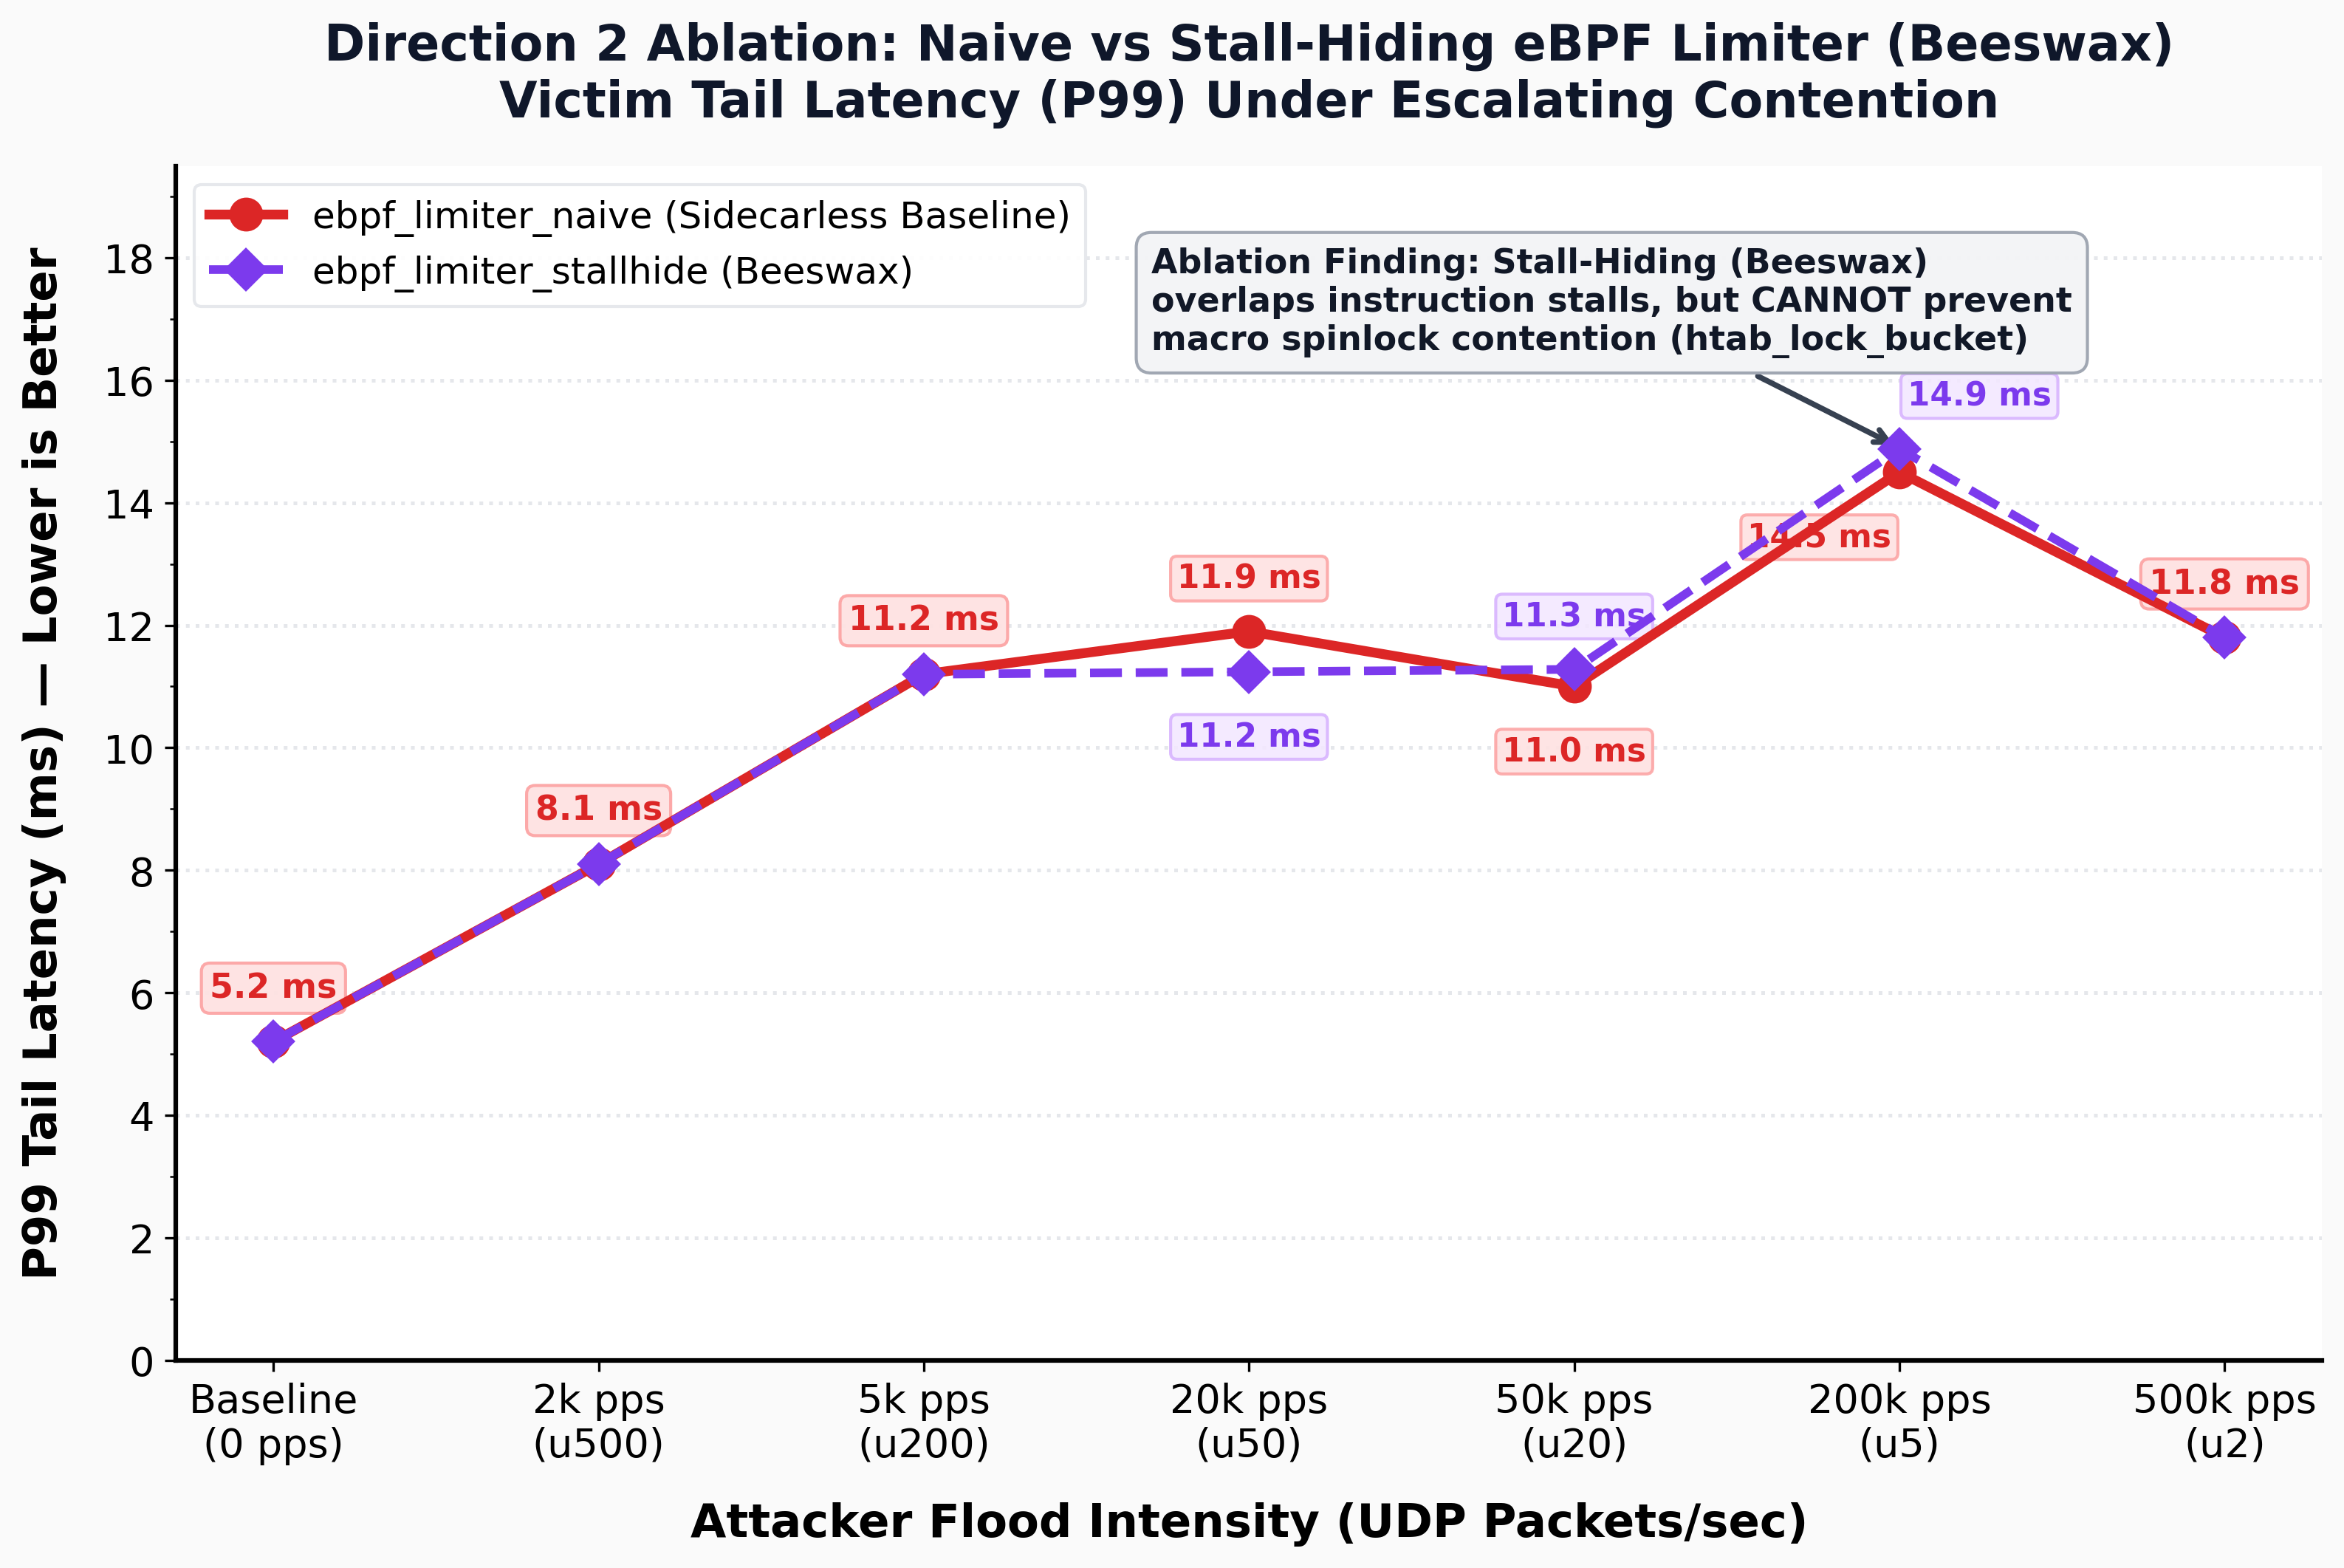
\includegraphics[width=0.8\textwidth]{images/Naive vs. Stall-Hiding Limiter Latency.png}
    \caption{Direction 2 Ablation: Naive vs. Stall-Hiding Limiter Latency}
    \label{fig:dir2_ablation}
\end{figure}

Early testing on Direction 1 suggested that the static priority-tier QoS
scheme worked reasonably well against a constant flood, but struggled once
the flood pattern changed over time -- which is closer to how real
noisy-neighbour traffic actually behaves. The dynamic rate limiter
tracked these changes more closely and showed better P99 latency in these
early tests (run at $N=2$ pilot trials for initial feasibility), which is why it was carried forward into the full evaluation
described in the next chapter. (These early comparisons were run at a
small sample size of $N=2$ pilot runs and are reported here only to explain why this direction
was chosen -- the statistically validated comparison across $N=10$ runs is presented
separately.)